\documentclass[12pt]{article}

%   Packages  
\usepackage[utf8]{inputenc}
\usepackage[margin=1in]{geometry}
\usepackage{amsmath, amssymb, amsfonts}
\usepackage{graphicx}
\usepackage{hyperref}
\usepackage{enumerate}
\usepackage{mathpazo}
\usepackage{float}

% --- Document Information ---
\title{18-799 Applied Computer Vision \\ Homework 1}
\author{\textbf{Name:} Edward Ajayi \\ \textbf{Andrew ID:} eaajayi \\ \textbf{Semester:} Spring 2026}
\date{\textbf{Date:} \today}

% Set the graphics path to the Assets folder
\graphicspath{{Assets/Assets/}}

\begin{document}

\maketitle
\newpage

\section*{Part I: Pinhole Camera Model}

\subsection*{Step 1: Define Camera and Image Plane Parameters}

\subsubsection*{(a) Image Plane Equations}

In this model, the image plane is the 2D surface where 3D points are projected. We define it in two ways:

\begin{enumerate}
    \item \textbf{Constant-depth plane ($Z = Z_0$):} \\
    In a standard setup where the camera center is $C = (C_x, C_y, C_z)$ and the focal length is $f$, the image plane is perpendicular to the optical axis (Z-axis). The equation is:
    \begin{equation}
        Z = C_z + f
    \end{equation}
    For our experiments, assuming $C = (0,0,0)$ and $f=50$, the equation is $Z = 50$.

    \item \textbf{A general plane:}
    \begin{equation}
        ax + by + cz + d = 0
    \end{equation}
    This is the general linear equation for a plane in 3D space. The coefficients $(a, b, c)$ represent the components of the normal vector $\mathbf{n}$ to the plane, which defines its orientation in space. The constant $d$ determines the plane's distance from the origin. This formulation is more flexible as it can represent a plane in any orientation, not just those perpendicular to a specific axis.
    
    For example, with $a=1$, $b=0$, $c=0.5$, and $d=50$:
    \begin{equation}
        1x + 0y + 0.5z + 50 = 0
    \end{equation}
\end{enumerate}

\subsubsection*{(b) Experimental Image Planes}
\begin{enumerate}
    \item \textbf{Standard Plane:} A plane perpendicular to the $Z$-axis. This uses the constant-depth equation $Z = Z_0$ (which is a special case of the general equation where $a=0$, $b=0$, $c=1$, and $d = -Z_0$, giving $0x + 0y + 1z - Z_0 = 0$). We choose $Z = f$, where the focal length $f$ is varied among 10, 50, and 100 for experimentation.
    \item \textbf{Slanted Plane:} A plane tilted relative to the optical axis. Using the general equation $1x + 0y + 0.5z + 50 = 0$, we can solve for depth as $z = -2x - 100$. This demonstrates that the depth $z$ is no longer constant but varies linearly based on the horizontal position $x$. Because the depth depends on $x$ but remains constant for all $y$ (since $b=0$), this simulates an image plane that has been rotated around the vertical $Y$-axis. This tilt causes perspective distortion, as one side of the image plane is physically closer to the scene than the other.
\end{enumerate}

\subsection*{Step 2: Trace Rays from 3D points to the Image Plane}

\subsubsection*{(a) Derivation of the Parametric Ray Equation}

In a pinhole camera model, light travels in a straight line from a scene point to the camera center. Mathematically, we model this as a ray originating from the camera center $C = (C_x, C_y, C_z)$ and passing through a 3D scene point $P = (X, Y, Z)$. 

To define the ray, we first calculate the direction vector $\mathbf{v} = \mathbf{P} - \mathbf{C}$. Any arbitrary point $\mathbf{L}(t)$ lying on this infinite line can be expressed by the parametric equation:
\begin{equation}
    \mathbf{L}(t) = \mathbf{C} + t(\mathbf{P} - \mathbf{C})
\end{equation}
Expanding this vector form into Cartesian components gives us the coordinates of any point along the light path as a function of the parameter $t$:
\begin{align}
    x(t) &= C_x + t(X - C_x) \nonumber \\
    y(t) &= C_y + t(Y - C_y) \\
    z(t) &= C_z + t(Z - C_z) \nonumber
\end{align}
In this formulation, $t$ acts as a scaling factor: $t=0$ yields the camera center ($C$), and $t=1$ yields the scene point ($P$). The intersection with the image plane will occur at a specific value of $t$ between these two bounds.

\subsubsection*{(b) Computing Ray-Plane Intersection}

The intersection point $I$ is defined as the unique point that simultaneously satisfies both the ray equations and the image plane equation $ax + by + cz + d = 0$. To find the specific value of $t$ at the moment of intersection, we substitute the expressions for $x(t)$, $y(t)$, and $z(t)$ into the plane equation:
\begin{equation}
    a(C_x + t(X - C_x)) + b(C_y + t(Y - C_y)) + c(C_z + t(Z - C_z)) + d = 0
\end{equation}
By distributing the coefficients and grouping terms containing $t$, we obtain:
\begin{equation}
    t[a(X - C_x) + b(Y - C_y) + c(Z - C_z)] + (aC_x + bC_y + cC_z + d) = 0
\end{equation}
Solving for $t$ allows us to find the exact ``distance'' along the ray where the light hits the image sensor:
\begin{equation}
    t = \frac{-(aC_x + bC_y + cC_z + d)}{a(X - C_x) + b(Y - C_y) + c(Z - C_z)}
\end{equation}
Once $t$ is known, it is substituted back into the equations in Step 2(a) to find the 3D coordinates of intersection point $I$.

\subsection*{Step 3: Project points onto the image plane}

Using the value of the parameter $t$ derived in the previous step, we can now determine the exact 3D coordinates where each ray intersects the image plane.

\subsubsection*{(a) Computation of Intersection Point $I$}

The intersection point $I$ represents the 3D location on the camera's sensor (image plane) that corresponds to the scene point $P$. Its coordinates depend on the type of image plane used:

\begin{enumerate}
    \item \textbf{For a Constant-Depth Plane ($Z = Z_0$):} \\
    In this standard configuration, the $Z$-coordinate of the intersection is pre-defined. The intersection point is:
    \begin{equation}
        I = (I_x, I_y, Z_0)
    \end{equation}
    where $I_x$ and $I_y$ are found by substituting the calculated $t$ into the ray equations:
    \begin{align}
        I_x &= C_x + t(X - C_x) \\
        I_y &= C_y + t(Y - C_y)
    \end{align}
    For our standard plane where $C = (0,0,0)$ and $Z_0 = f$, we can derive $t$ directly. Since the plane equation is $Z = f$ (or equivalently $0x + 0y + 1z - f = 0$), we have:
    \[
    t = \frac{f - C_z}{Z - C_z} = \frac{f}{Z}
    \]
    Therefore, the intersection coordinates simplify to:
    \[
    I_x = \frac{fX}{Z}, \quad I_y = \frac{fY}{Z}
    \]
    This is the classic perspective projection formula.

    \item \textbf{For a Tilted Plane ($ax + by + cz + d = 0$):} \\
    For a tilted plane, the intersection point $I = (I_x, I_y, I_z)$ must satisfy the plane equation. Here, the $Z$-coordinate is not constant and must be computed alongside $X$ and $Y$ using the parameter $t$:
    \begin{align}
        I_x &= C_x + t(X - C_x) \\
        I_y &= C_y + t(Y - C_y) \\
        I_z &= C_z + t(Z - C_z)
    \end{align}
\end{enumerate}

\subsubsection*{(b) Iterative Projection for all 3D points}

This intersection calculation is repeated iteratively for every 3D point in the provided dataset. We perform this process separately for each defined image plane (the standard perpendicular plane and the tilted/slanted plane) to compare how the plane's orientation affects the distribution of projected points.

Figure~\ref{fig:focal} shows the projection results for all 3D points onto the standard plane $Z = f$ with three different focal lengths ($f = 10, 50, 100$). Figure~\ref{fig:tilted} shows the projection onto the tilted plane.

\subsection*{Step 4: Map Projected Points to 2D Image Coordinates}

\subsubsection*{(a) Mapping Equations}

The 3D intersection point $I = (I_x, I_y, I_z)$ on the image plane must be converted to 2D pixel coordinates $(u, v)$. The general mapping equation is:
\begin{equation}
    u = s_x(I_x - O_x) + c_x, \quad v = s_y(I_y - O_y) + c_y
\end{equation}

where:
\begin{itemize}
    \item $(c_x, c_y)$ is the \textbf{principal point}    the pixel coordinates where the optical axis intersects the image plane. This shifts the origin of the projection from the corner to the center of the image.
    \item $s_x, s_y$ are the \textbf{pixel scaling factors}    these convert from physical units (e.g., millimeters) to pixel units. They account for non-square pixels if the sensor has different horizontal and vertical pixel densities.
    \item $(O_x, O_y)$ is the \textbf{origin offset} on the image plane.
\end{itemize}

Following the assignment assumptions ($O_x = O_y = 0$ and $s_x = s_y = 1$), we substitute into the general equation:
\begin{align}
    u &= 1 \cdot (I_x - 0) + c_x = I_x + c_x \\
    v &= 1 \cdot (I_y - 0) + c_y = I_y + c_y
\end{align}

For our implementation, we set $(c_x, c_y) = (0, 0)$, so the final mapping is:
\begin{equation}
    u = I_x, \quad v = I_y
\end{equation}

\subsubsection*{(b) Compute $(u, v)$ for all projected points}

We applied the mapping equation to all intersection points computed in Step 3. For each 3D point in the blue and black point datasets:

\begin{enumerate}
    \item Compute the intersection point $I = (I_x, I_y)$ on the image plane (from Step 3)
    \item Apply the mapping: $u = I_x + c_x$, $v = I_y + c_y$
    \item Since $c_x = c_y = 0$: $(u, v) = (I_x, I_y)$
\end{enumerate}

This was repeated for all three focal lengths ($f = 10, 50, 100$), producing three sets of 2D image coordinates for the standard plane, plus one set for the tilted plane. The results are visualized in Figures~\ref{fig:focal} and~\ref{fig:tilted}.

\subsection*{Experimental Results}

\subsubsection*{Projection with a Standard Image Plane (Focal Length Comparison)}

Figure~\ref{fig:focal} shows how changing focal length affects the projected image. Experiments were conducted with $f = 10, 50, 100$ using the standard plane $Z = f$. Longer focal lengths produce a ``zoom'' effect  points spread further from the center, making the scene appear larger.

\begin{figure}[H]
    \centering
    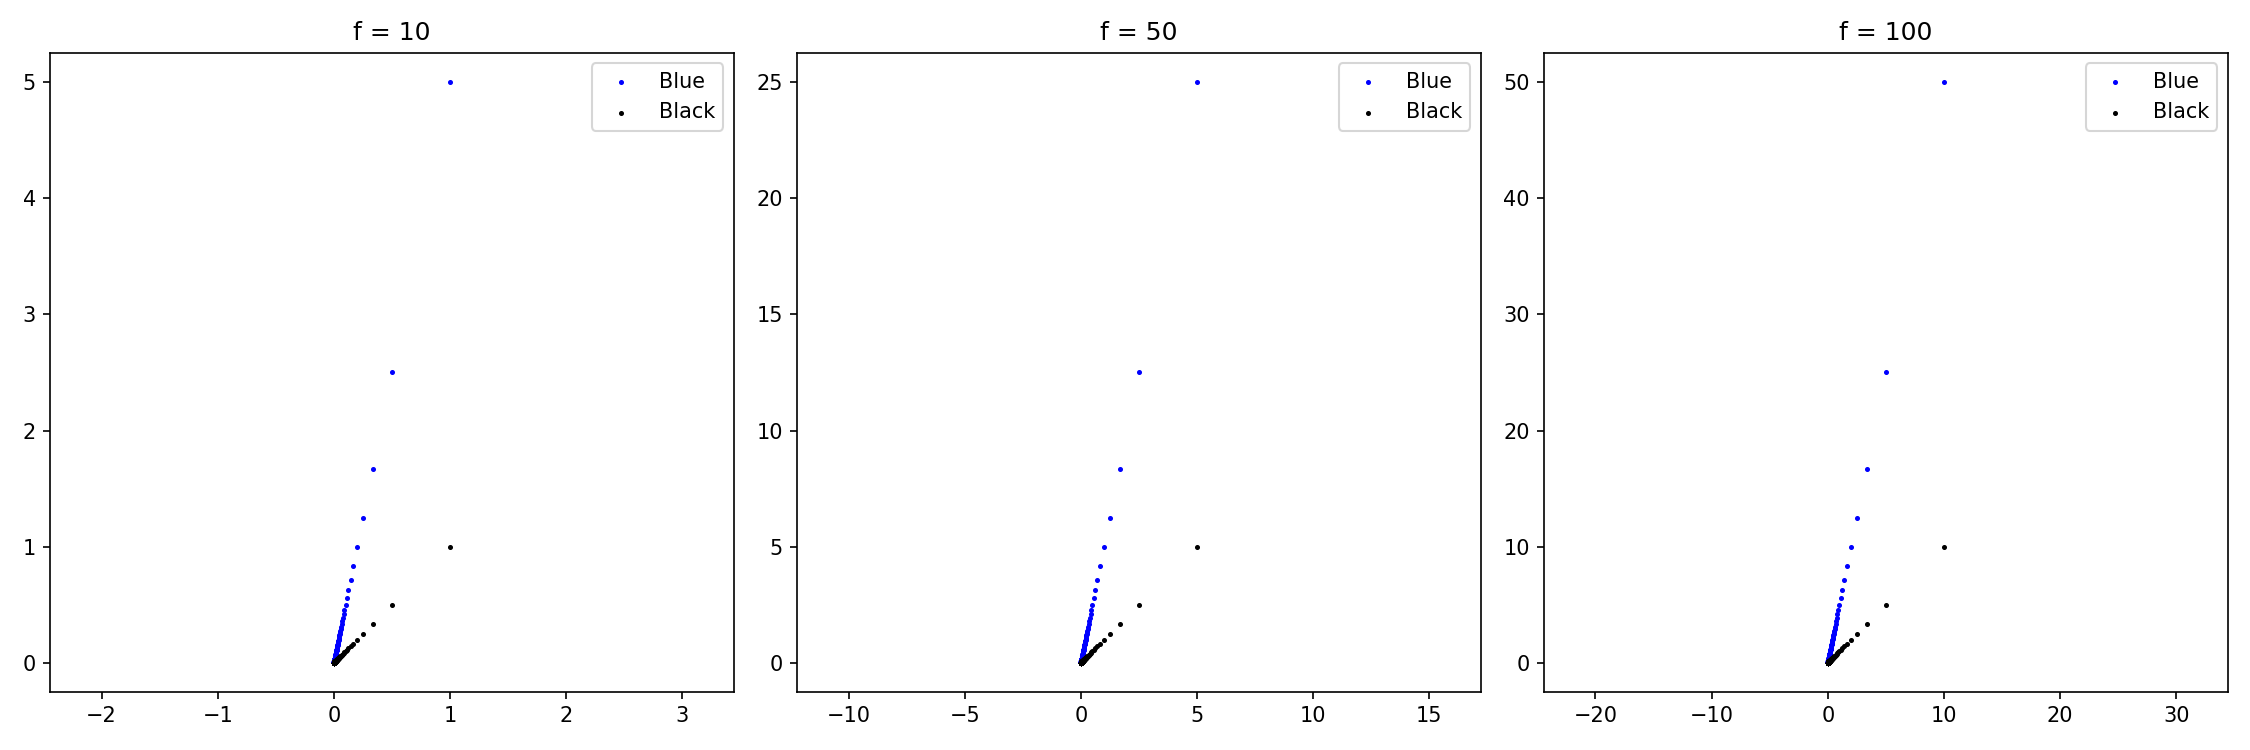
\includegraphics[width=0.95\textwidth]{focal_length_comparison.png}
    \caption{Projection results for $f = 10, 50, 100$. Notice how larger $f$ magnifies the projection. At $f=10$, points are clustered near the center. At $f=100$, the same points spread across a much larger area.}
    \label{fig:focal}
\end{figure}

\subsubsection*{Projection with a Tilted Image Plane}

Figure~\ref{fig:tilted} shows projection onto a tilted plane defined by $0.1x + 0y + 1z - 50 = 0$. The asymmetric distortion is visible---one side appears stretched compared to the other because that side of the image plane is further from the scene.

\begin{figure}[H]
    \centering
    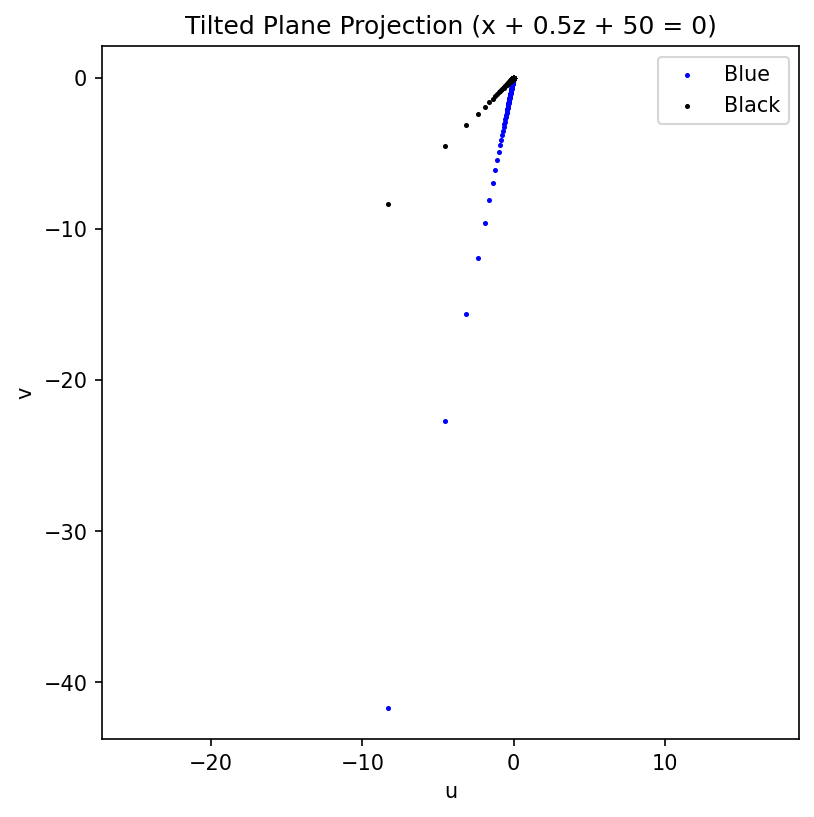
\includegraphics[width=0.5\textwidth]{tilted_plane_projection.png}
    \caption{Projection onto tilted plane $0.1x + 1z - 50 = 0$. The keystoning effect is visible---the left side is compressed while the right side is expanded.}
    \label{fig:tilted}
\end{figure}

\subsection*{Analysis of Parameters}

\subsubsection*{Effect of Focal Length on Projected Image}

Increasing the focal length $f$ increases the distance between the camera center and the image plane. This causes the projected points to be scaled outward from the principal point, effectively ``zooming in'' on the scene. Mathematically, from the projection formula $I_x = fX/Z$, we see that $f$ acts as a direct scaling factor. Doubling $f$ doubles the projected coordinates, spreading points further apart.

Looking at Figure~\ref{fig:focal}, as $f$ goes from 10 to 100, the projected points spread further apart. This is because the image plane moves further from the camera, so rays have more distance to diverge before hitting it.

\subsubsection*{Influence of Image Plane Position and Orientation}

The image plane's position (distance from camera) determines the scale of the projection. Its orientation affects how depth maps to image coordinates:
\begin{itemize}
    \item \textbf{Standard plane:} All points at the same depth $Z$ project with the same scaling factor $f/Z$
    \item \textbf{Tilted plane:} The effective ``focal length'' varies across the image. Points on the side tilted toward the camera have a smaller effective distance and project smaller. Points on the side tilted away have a larger effective distance and project larger.
\end{itemize}

A tilted plane causes keystoning (perspective distortion)---one side of the scene appears compressed while the other stretches out, as seen in Figure~\ref{fig:tilted}. This is the same effect seen when a projector is not perpendicular to the screen.

\subsubsection*{Comparison of Standard vs. Tilted Plane Projections}

The standard plane ($Z = f$) produces symmetric projections where distortion depends only on depth. The tilted plane introduces asymmetric distortion: points on one side (closer to the plane) project smaller, while points on the other side (further from the plane) project larger. This creates the trapezoidal ``keystone'' shape.

\subsection*{Ideal Points and Distance Analysis}

We computed the Euclidean (L2) distances between corresponding black and blue points before and after projection (using $f = 50$):

\begin{center}
\begin{tabular}{|l|c|c|}
\hline
\textbf{Point Pair} & \textbf{3D Distance (Before Projection)} & \textbf{2D Distance (After Projection)} \\
\hline
First black \& first blue point & 4.0000 & 20.0000 \\
\hline
Last black \& last blue point & 4.0000 & 0.0000 \\
\hline
\end{tabular}
\end{center}

\subsubsection*{Observations}

\begin{enumerate}
    \item The \textbf{first pair} of points had a 3D distance of 4.0, but after projection the 2D distance became 20.0 --- the distance \textbf{increased} by a factor of 5.
    \item The \textbf{last pair} of points also had a 3D distance of 4.0, but after projection the 2D distance became 0.0 --- the points \textbf{collapsed} to the same location!
    \item Even though both pairs had \textbf{identical 3D distances} (4.0), their 2D distances are completely different (20.0 vs 0.0).
\end{enumerate}

This clearly demonstrates that Euclidean distances are \textbf{not preserved} after perspective projection.

\subsubsection*{Why Distances Are Not Preserved}

Distances are \textbf{not preserved} because perspective projection is a nonlinear transformation. Each 3D point $(X, Y, Z)$ gets scaled by $1/Z$ during projection:
\[
(u, v) = \left(\frac{fX}{Z}, \frac{fY}{Z}\right)
\]
Since each point has a different $Z$-coordinate, they get scaled by different factors. The key insight is:
\begin{enumerate}
    \item Two points at the same 3D distance will have different 2D distances unless they happen to be at exactly the same depth
    \item A point closer to the camera (smaller $Z$) projects larger than a point farther away (larger $Z$)
    \item The depth-dependent scaling $1/Z$ is what creates the ``near things look big, far things look small'' effect of perspective
\end{enumerate}

This non-preservation of distances is fundamental to perspective projection and is why parallel lines appear to converge at vanishing points in photographs.

\newpage
\section*{Part II: Rendering Views from a 3D Point Cloud}

In this part, the pinhole camera model from Part I  was extended to render a complete 3D point cloud from multiple viewpoints. The objective is to simulate how video games and 3D simulators generate images by moving a virtual camera through a static 3D world.

For this experiment, a 3D point cloud was loaded (\texttt{scene.ply}, containing 314,016 points) and rendered it from six different camera positions \textbf{without rotating the point cloud itself}. All changes in the rendered images result solely from changes in the camera position and orientation.

\subsection*{Step 5: Define Camera Poses}

\subsubsection*{(a) Define a consistent world coordinate system for the point cloud}

To establish a consistent coordinate system, the centroid (center of mass) of all points in the point cloud was first computed:
\[
\mathbf{centroid} = \frac{1}{N} \sum_{i=1}^{N} \mathbf{P}_i
\]
where $N$ is the total number of points. The world origin was then defined at this centroid so that the scene is centered at $(0, 0, 0)$. This centering ensures that when cameras are placed around the scene, they are equidistant from the center of the object.

The camera distance $d$ was set to $3 \times$ the maximum extent of the point cloud (the largest distance from the centroid to any point) to ensure all points are visible from every viewpoint without clipping.

\subsubsection*{(b) Specify camera centers and orientations for all six views}

For each viewpoint, a camera pose is defined consisting of:
\begin{itemize}
    \item \textbf{Camera center $\mathbf{C}$}: The 3D position of the camera in world coordinates
    \item \textbf{Rotation matrix $\mathbf{R}$}: A $3 \times 3$ orthogonal matrix that transforms points from world coordinates to camera coordinates
\end{itemize}

The complete transformation from world to camera coordinates is:
\begin{equation}
    \mathbf{P}_{cam} = \mathbf{R}(\mathbf{P}_{world} - \mathbf{C})
\end{equation}

This transformation has two steps:
\begin{enumerate}
    \item \textbf{Translation:} $(\mathbf{P}_{world} - \mathbf{C})$ shifts all points so the camera is at the origin
    \item \textbf{Rotation:} $\mathbf{R}$ rotates the scene so the camera looks down the positive $Z_c$ axis
\end{enumerate}

Here are the six camera setups (positions relative to the centroid):

\begin{center}
\begin{tabular}{|l|c|l|}
\hline
\textbf{View} & \textbf{Camera Position $\mathbf{C}$} & \textbf{Looking Toward} \\
\hline
Front & $(0, 0, +d)$ & $-Z$ direction (into the scene) \\
Back & $(0, 0, -d)$ & $+Z$ direction (toward positive Z) \\
Left & $(-d, 0, 0)$ & $+X$ direction (toward positive X) \\
Right & $(+d, 0, 0)$ & $-X$ direction (toward negative X) \\
Top & $(0, +d, 0)$ & $-Y$ direction (looking down) \\
Bottom & $(0, -d, 0)$ & $+Y$ direction (looking up) \\
\hline
\end{tabular}
\end{center}

\subsubsection*{(c) Clearly state the viewing direction for each camera}

Each rotation matrix $\mathbf{R}$ is constructed so that after transformation, points in front of the camera have positive $Z_c$ (required for perspective projection to work correctly). The rotation matrices for each view are:

\textbf{Front View:} Camera at $(0, 0, +d)$, looking toward $-Z$
\[
\mathbf{R}_{front} = \begin{pmatrix} 1 & 0 & 0 \\ 0 & 1 & 0 \\ 0 & 0 & -1 \end{pmatrix}
\]
This flips the Z-axis so points originally at positive Z (behind the camera) become negative $Z_c$.

\textbf{Back View:} Camera at $(0, 0, -d)$, looking toward $+Z$
\[
\mathbf{R}_{back} = \begin{pmatrix} -1 & 0 & 0 \\ 0 & 1 & 0 \\ 0 & 0 & 1 \end{pmatrix}
\]

\textbf{Left View:} Camera at $(-d, 0, 0)$, looking toward $+X$
\[
\mathbf{R}_{left} = \begin{pmatrix} 0 & 0 & 1 \\ 0 & 1 & 0 \\ -1 & 0 & 0 \end{pmatrix}
\]

\textbf{Right View:} Camera at $(+d, 0, 0)$, looking toward $-X$
\[
\mathbf{R}_{right} = \begin{pmatrix} 0 & 0 & -1 \\ 0 & 1 & 0 \\ 1 & 0 & 0 \end{pmatrix}
\]

\textbf{Top View:} Camera at $(0, +d, 0)$, looking toward $-Y$
\[
\mathbf{R}_{top} = \begin{pmatrix} 1 & 0 & 0 \\ 0 & 0 & -1 \\ 0 & 1 & 0 \end{pmatrix}
\]

\textbf{Bottom View:} Camera at $(0, -d, 0)$, looking toward $+Y$
\[
\mathbf{R}_{bottom} = \begin{pmatrix} 1 & 0 & 0 \\ 0 & 0 & 1 \\ 0 & -1 & 0 \end{pmatrix}
\]

\subsection*{Step 6: Perspective Projection of the Point Cloud}

\subsubsection*{(a) Project all visible points onto the image plane}

For each camera pose, the following steps are performed for every point:

\begin{enumerate}
    \item \textbf{Transform to camera coordinates:}
    \[
    \begin{pmatrix} X_c \\ Y_c \\ Z_c \end{pmatrix} = \mathbf{R} \left( \begin{pmatrix} X_w \\ Y_w \\ Z_w \end{pmatrix} - \mathbf{C} \right)
    \]
    
    \item \textbf{Filter points behind the camera:} Discard any point where $Z_c \leq 0$. These points are behind the camera and cannot be seen.
    
    \item \textbf{Apply perspective projection:}
    \begin{equation}
        u = f \cdot \frac{X_c}{Z_c}, \quad v = f \cdot \frac{Y_c}{Z_c}
    \end{equation}
    where $f$ is the focal length ($f = 500$ was used for all views).
\end{enumerate}

\subsubsection*{(b) Map the projected points to 2D image coordinates}

The projected coordinates $(u, v)$ are then shifted by the principal point $(c_x, c_y)$ to center the image:
\[
u_{pixel} = u + c_x, \quad v_{pixel} = v + c_y
\]
The principal point $(c_x, c_y)$ was set to the center of the image grid to ensure the projection is centered in the output image.

\subsection*{Step 7: Image Formation}

For image formation, a 2D image grid of fixed resolution was created (e.g., $800 \times 600$ pixels) for all views. Each projected point is plotted at its corresponding $(u_{pixel}, v_{pixel})$ location. When multiple 3D points project to the same pixel, the point with smaller $Z_c$ (closer to camera) takes precedence (depth buffering).

Figure~\ref{fig:sixviews} shows all six rendered views. A focal length of $f = 500$ and consistent image dimensions were used across all views.

\begin{figure}[H]
    \centering
    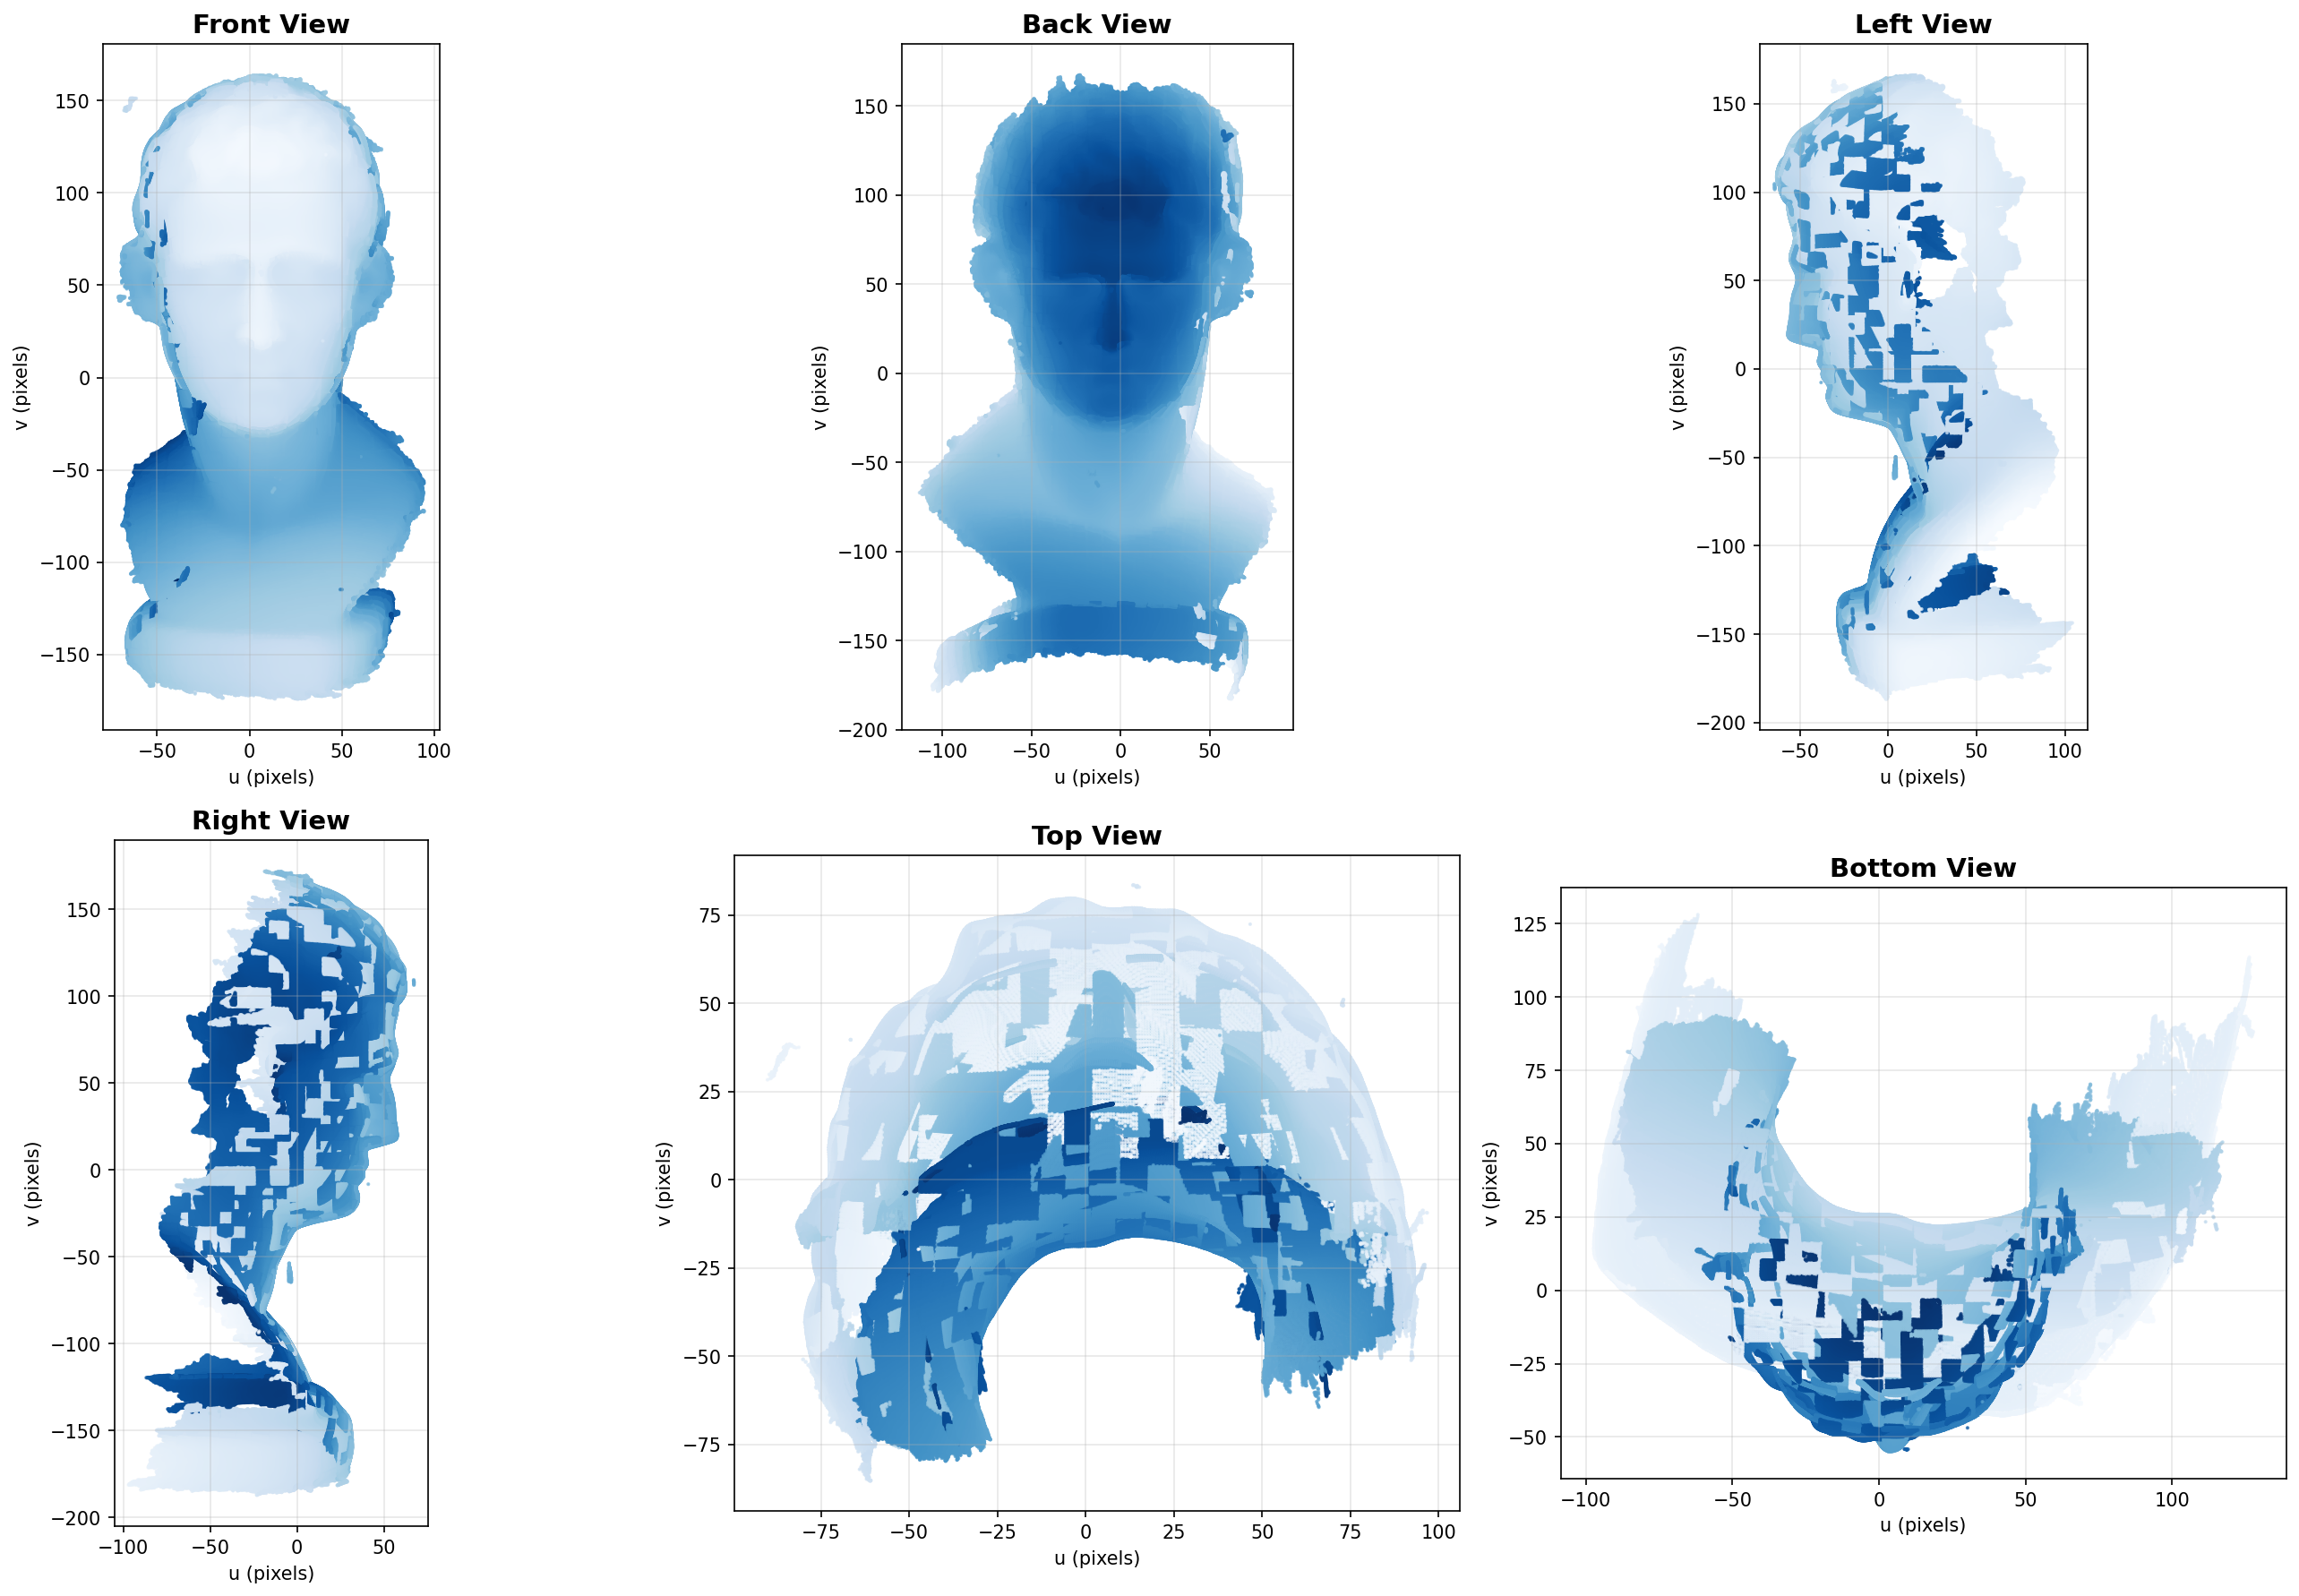
\includegraphics[width=0.95\textwidth]{part2_six_views.png}
    \caption{Six canonical views of the 3D point cloud. Each view shows the scene from a different camera position: Front, Back, Left, Right, Top, and Bottom. Notice how the same 3D scene appears completely different depending on the viewing angle.}
    \label{fig:sixviews}
\end{figure}

\subsection*{Custom Scene (ReVo 3D Camera)}

ReVo 3D camera was used to capture a custom scene with a different object. The file contains 782,706 points. The same six-view rendering pipeline was applied to this custom point cloud. Figure~\ref{fig:custom} shows the results.

\begin{figure}[H]
    \centering
    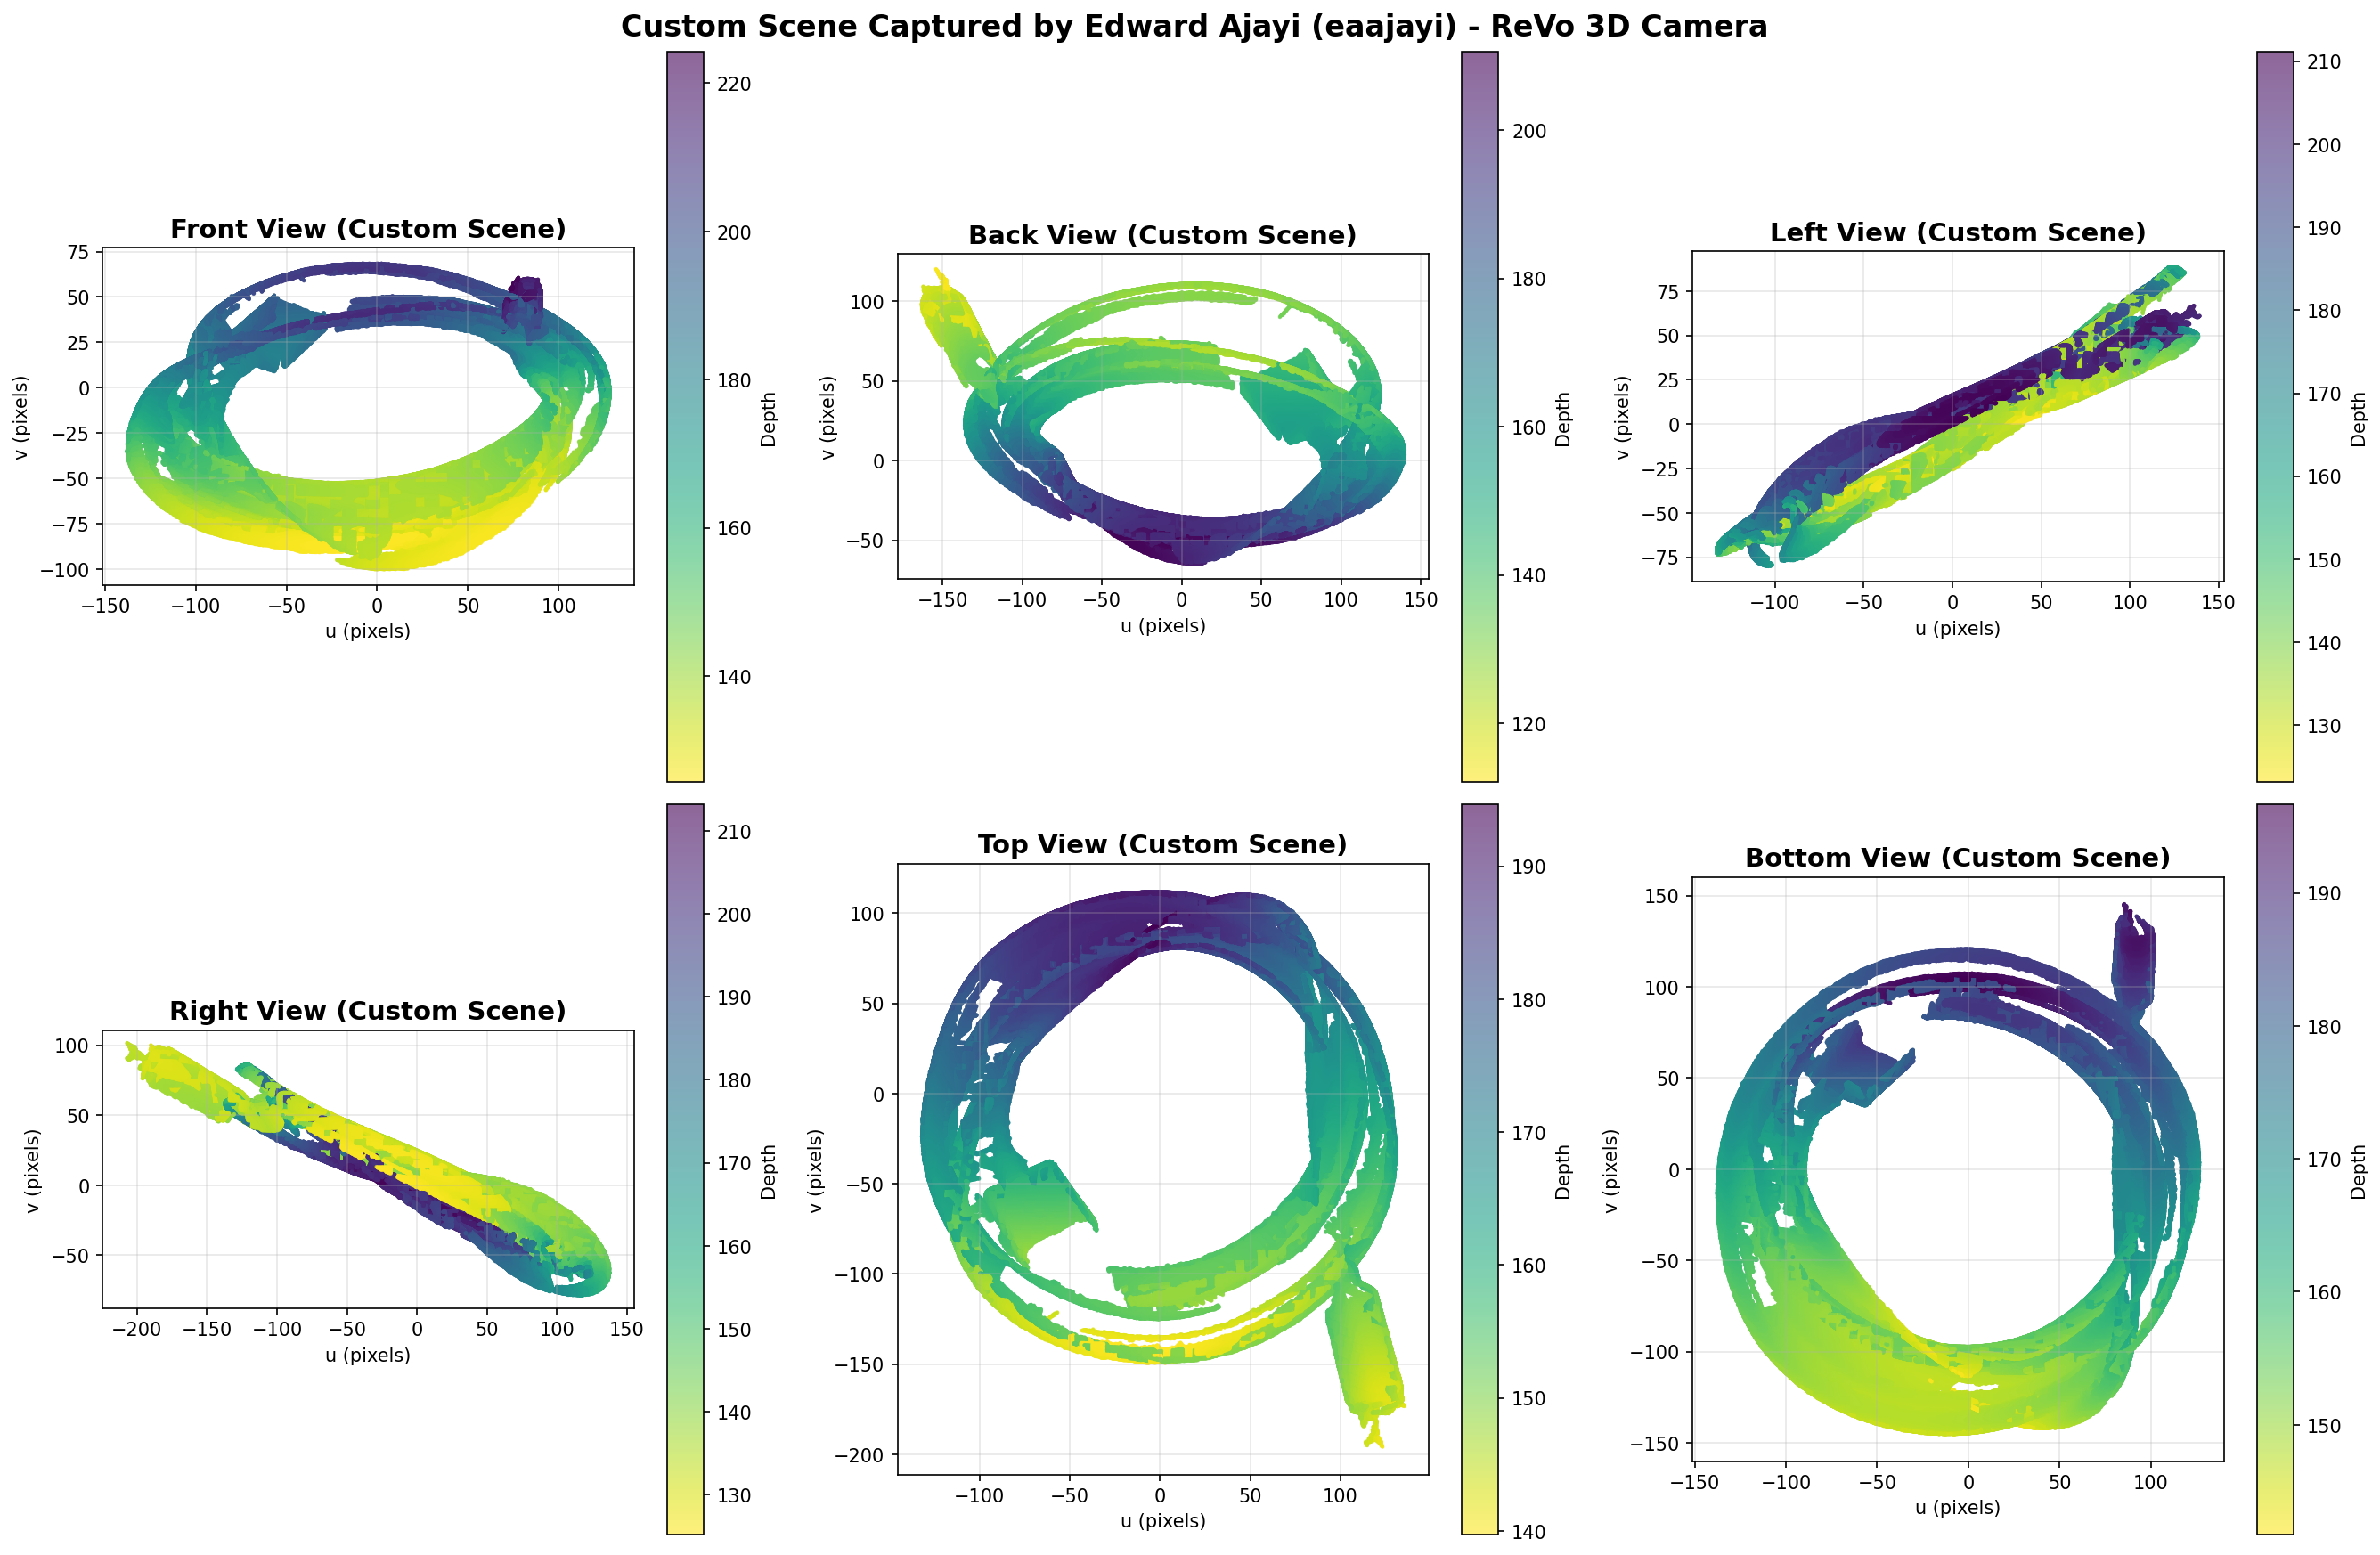
\includegraphics[width=0.95\textwidth]{part2_custom_scene_six_views.png}
    \caption{Six views of the custom captured scene using the ReVo 3D camera. The same rendering pipeline was applied to demonstrate generalization to different point clouds.}
    \label{fig:custom}
\end{figure}

\subsection*{Analysis Questions}

\subsubsection*{How Changing Camera Pose Produces Different Images}

Changing the camera pose alone produces different images of the same 3D scene because the projection depends entirely on where we view from. The 3D point cloud never moves as it stays fixed in world coordinates. What changes is:
\begin{enumerate}
    \item \textbf{Camera position $\mathbf{C}$}: This determines which points are ``in front'' (visible) vs. ``behind'' (invisible). It also affects the relative distances from the camera to each point, which impacts perspective scaling.
    \item \textbf{Camera orientation $\mathbf{R}$}: This rotates our viewing direction, determining which surfaces of objects face the camera and which are turned away.
\end{enumerate}

The transformation $\mathbf{P}_{cam} = \mathbf{R}(\mathbf{P}_{world} - \mathbf{C})$ first translates the world so the camera is at the origin, then rotates so the camera looks down the positive $Z_c$ axis. Different $(\mathbf{C}, \mathbf{R})$ pairs give us the six different views in Figure~\ref{fig:sixviews}.

\subsubsection*{Effect of Camera Orientation on Perceived Scene Structure}

The rotation matrix $\mathbf{R}$ fundamentally changes how we perceive the 3D structure of the scene:
\begin{itemize}
    \item \textbf{Visibility:} Different orientations reveal different surfaces. From the Front view, one side of the object is visible but not the back. From the Top view, the object is seen from above, revealing the overall layout on the scanning plate.
    \item \textbf{Occlusion:} Parts of the object can hide behind other parts. A section of the USB wire visible from the Front may be occluded by another section when viewed from the Left.
    \item \textbf{Shape perception:} The wire's 3D curvature is perceived differently from each angle. From one view it may appear straight, while from another angle the bends and curves become visible.
\end{itemize}

This is why 3D applications allow camera rotation: no single view captures all the structural information of a 3D scene.

\subsubsection*{Why Perspective Distortion Varies Across Views}

Perspective distortion arises from the $1/Z_c$ term in projection. The amount and pattern of distortion depends on how depth ($Z_c$) varies across the scene from each camera's perspective:

\begin{itemize}
    \item \textbf{Top View:} When looking straight down at the object, surfaces facing upward appear at roughly constant depth. This produces minimal perspective distortion the image looks almost like an orthographic (map-like) projection.
    \item \textbf{Front/Side Views:} The object has varying depth from these angles. Parts of the object closer to the camera appear larger than parts farther away, creating the classic perspective effect where near things look big and far things look small.
    \item \textbf{Asymmetric objects:} The USB wire scanned on the 3D scanning plate is not a symmetric object it curves and extends more in some directions than others. Each viewpoint produces a different distortion pattern based on how the depth is distributed from that angle.
\end{itemize}

\subsubsection*{Relation to Camera Navigation in Video Games and Simulators}

This experiment replicates exactly what happens in real-time 3D graphics engines used in video games, flight simulators, and virtual reality applications:

\begin{enumerate}
    \item \textbf{Static 3D World:} The game world (level geometry, objects, characters) is stored as fixed vertex data in GPU memory. This data never changes when the player moves only the camera changes.
    
    \item \textbf{Virtual Camera:} The player's viewpoint is represented as a virtual camera with position $\mathbf{C}$ and orientation $\mathbf{R}$ (often stored as a quaternion for smooth interpolation).
    
    \item \textbf{Real-time Transformation:} Every frame (typically 60 times per second), the graphics engine:
    \begin{itemize}
        \item Computes $\mathbf{P}_{cam} = \mathbf{R}(\mathbf{P}_{world} - \mathbf{C})$ for all vertices
        \item Applies perspective projection: $u = f \cdot X_c/Z_c$, $v = f \cdot Y_c/Z_c$
        \item Rasterizes triangles and applies textures/shading
    \end{itemize}
    
    \item \textbf{This Experiment:} The six static views of the USB wire are equivalent to six screenshots where a virtual camera was placed at six fixed positions around the object. The mathematics is identical game engines just do it faster (millions of vertices at 60+ FPS using GPU parallelism).
\end{enumerate}

This connection highlights why understanding the pinhole camera model is fundamental to computer graphics, robotics, augmented reality, and any application that involves rendering 3D scenes onto 2D displays.

\newpage
\section*{Part III: Image Demosaicing}

\subsection*{Background: The Bayer Filter and Color Filter Arrays}

Digital camera sensors are inherently monochromatic each pixel measures only the intensity of light, not its color. To capture color images, most cameras use a \textbf{Color Filter Array (CFA)}, with the \textbf{Bayer pattern} being the most common. In a Bayer filter, each pixel is covered by a colored filter that allows only one color (Red, Green, or Blue) to pass through:

\begin{center}
\begin{tabular}{|c|c|c|c|c|c|}
\hline
R & G & R & G & R & G \\
\hline
G & B & G & B & G & B \\
\hline
R & G & R & G & R & G \\
\hline
G & B & G & B & G & B \\
\hline
\end{tabular}
\end{center}

Notice that:
\begin{itemize}
    \item Green pixels appear twice as often as Red or Blue (50\% Green, 25\% Red, 25\% Blue)
    \item This matches human vision, which is most sensitive to green light
    \item At each pixel location, only \textbf{one} color channel is measured; the other two are \textbf{missing}
\end{itemize}

The challenge is to reconstruct a full RGB image where every pixel has all three color values. This process is called \textbf{demosaicing} (also spelled ``demosaicking'').

\subsection*{Implementation: Bilinear Interpolation}

The \textbf{bilinear interpolation} algorithm was implemented, which estimates missing color values by averaging neighboring pixels of the same color. The approach differs based on which color is present at each pixel:

\subsubsection*{Algorithm Details}

\begin{enumerate}
    \item \textbf{At a Red pixel $(i, j)$:}
    \begin{itemize}
        \item Red is known: $R(i,j)$ is the measured value
        \item Green is estimated from 4 horizontal/vertical neighbors:
        \[
        G(i,j) = \frac{G(i-1,j) + G(i+1,j) + G(i,j-1) + G(i,j+1)}{4}
        \]
        \item Blue is estimated from 4 diagonal neighbors:
        \[
        B(i,j) = \frac{B(i-1,j-1) + B(i-1,j+1) + B(i+1,j-1) + B(i+1,j+1)}{4}
        \]
    \end{itemize}
    
    \item \textbf{At a Blue pixel $(i, j)$:}
    \begin{itemize}
        \item Blue is known: $B(i,j)$ is the measured value
        \item Green is estimated from 4 horizontal/vertical neighbors (same as above)
        \item Red is estimated from 4 diagonal neighbors (same formula as Blue at Red pixel)
    \end{itemize}
    
    \item \textbf{At a Green pixel $(i, j)$:}
    \begin{itemize}
        \item Green is known: $G(i,j)$ is the measured value
        \item Depending on the row, either Red or Blue is on the same row:
        \begin{itemize}
            \item If Red is on the same row: $R(i,j) = \frac{R(i,j-1) + R(i,j+1)}{2}$ and $B(i,j) = \frac{B(i-1,j) + B(i+1,j)}{2}$
            \item If Blue is on the same row: $B(i,j) = \frac{B(i,j-1) + B(i,j+1)}{2}$ and $R(i,j) = \frac{R(i-1,j) + R(i+1,j)}{2}$
        \end{itemize}
    \end{itemize}
    
    \item \textbf{Boundary handling:} At image edges where not all neighbors exist, only the available neighbors are used for averaging.
\end{enumerate}

\subsubsection*{Results}

Figure~\ref{fig:demosaic} shows the demosaiced result from raw Bayer data.

\begin{figure}[H]
    \centering
    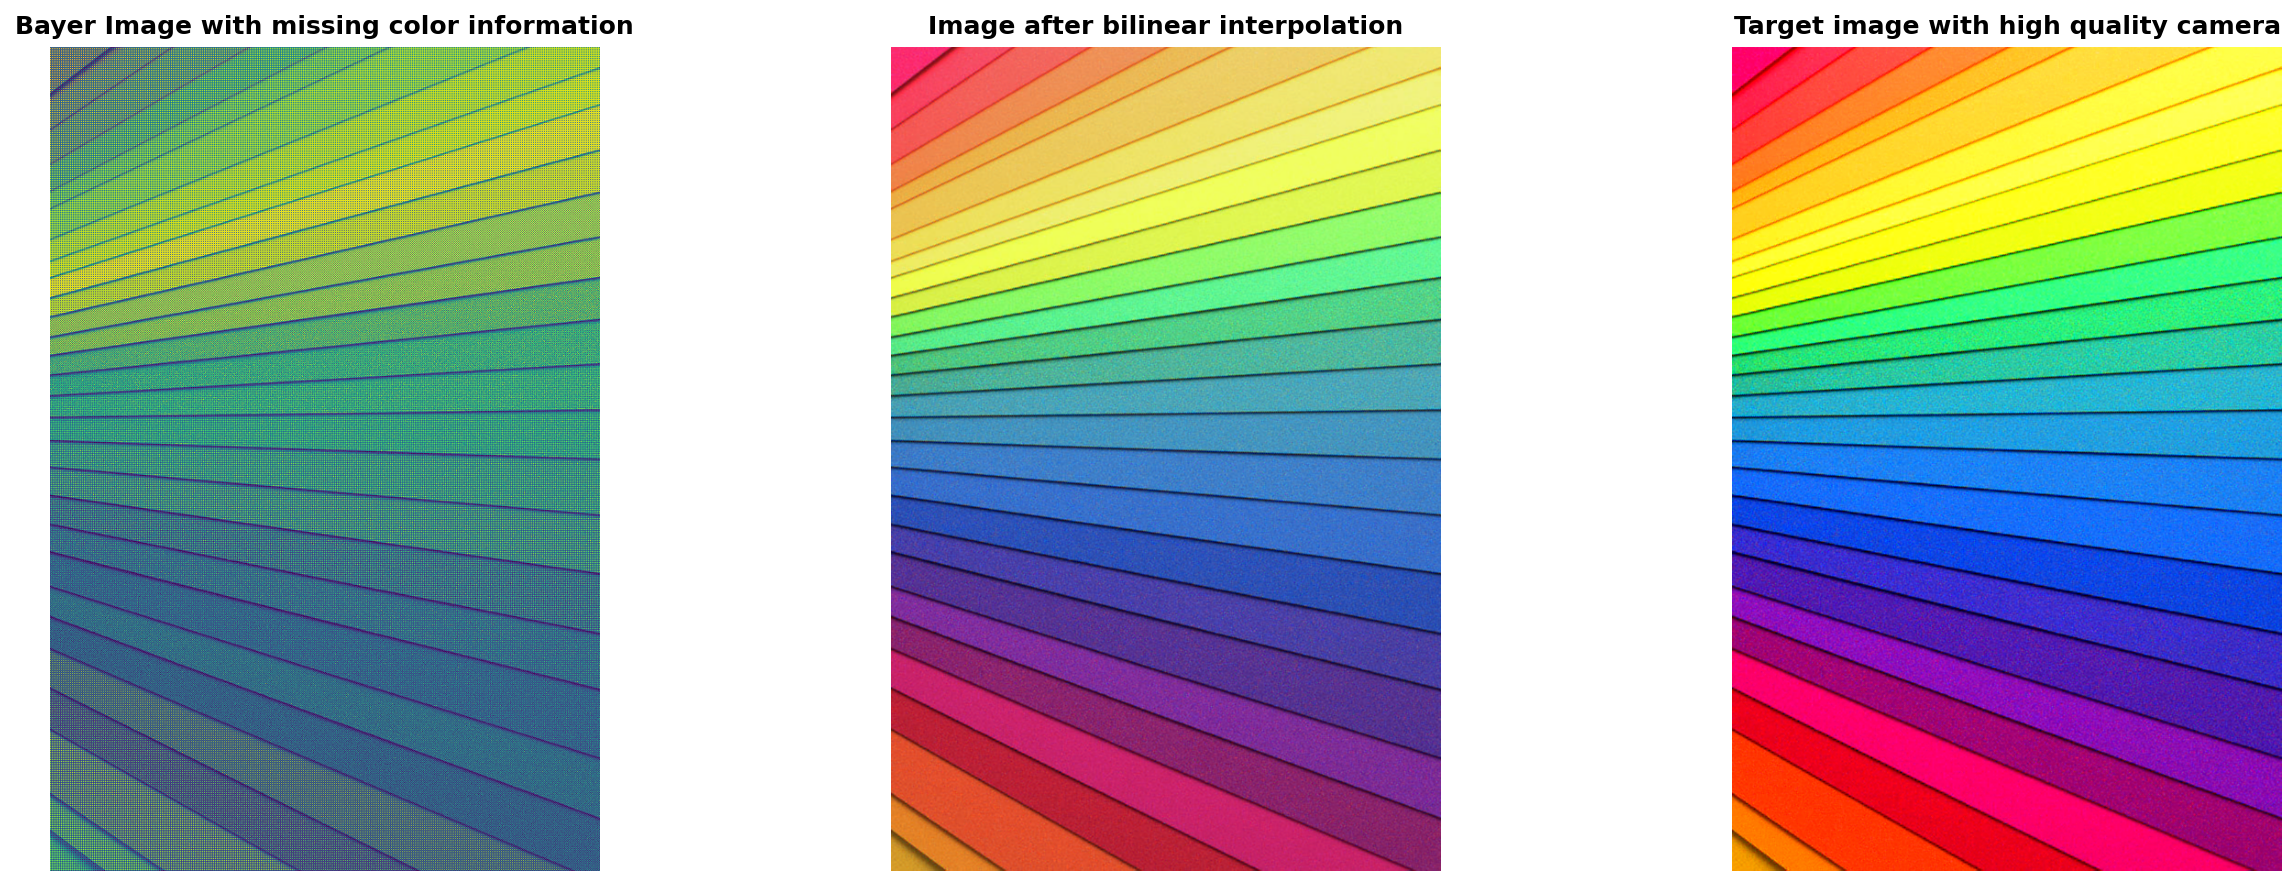
\includegraphics[width=0.6\textwidth]{demosaiced_result.png}
    \caption{Demosaiced RGB image from raw Bayer data using bilinear interpolation. The algorithm successfully reconstructs a full-color image from the single-channel Bayer pattern.}
    \label{fig:demosaic}
\end{figure}

\subsection*{Limitations of Bilinear Interpolation}

While bilinear interpolation is simple and fast, it has significant limitations:

\begin{enumerate}
    \item \textbf{Edge Blurring:} When averaging across a sharp edge, the algorithm mixes colors from both sides of the edge, resulting in blurred transitions. For example, at a boundary between a red object and a blue background, the estimated values will contain unwanted mixing.
    
    \item \textbf{Color Fringing (Chromatic Artifacts):} At high-contrast edges, especially diagonal ones, false colors appear as ``halos'' or ``zippering'' patterns. This occurs because the algorithm assumes colors vary smoothly, which is violated at edges.
    
    \item \textbf{Loss of Fine Details:} Small patterns (especially those with spatial frequencies near the Nyquist limit of the sensor) get smoothed out. Features smaller than 2-3 pixels may be lost entirely.
    
    \item \textbf{Moir\'e Patterns:} When the scene contains regular patterns (like fabric textures or building facades), bilinear interpolation can produce interference patterns not present in the original scene.
\end{enumerate}

\subsection*{Potential Improvements}

Several approaches can improve demosaicing quality:

\begin{itemize}
    \item \textbf{Edge-Directed Interpolation:} Before interpolating, detect the direction of edges using gradient analysis. Then interpolate \textbf{along} edges rather than across them. This preserves edge sharpness while still filling in missing colors.
    
    \item \textbf{Adaptive Weighting:} Use different interpolation strategies for different regions:
    \begin{itemize}
        \item In smooth regions: simple averaging works well
        \item Near edges: weight neighbors based on similarity to avoid mixing across edges
        \item Use local variance or gradient magnitude to decide which strategy to apply
    \end{itemize}
    
    \item \textbf{Constant Hue Assumption:} Many advanced algorithms (like the Malvar-He-Cutler method) exploit the observation that the \textit{ratio} between color channels often varies more slowly than the absolute values. By interpolating color differences or ratios rather than colors directly, edges are preserved better.
\end{itemize}

\subsection*{Alternative Demosaicing Algorithms}

\begin{itemize}
    \item \textbf{Nearest Neighbor:} Simply copies the nearest pixel of each color\cite{shakhnarovich2008nearest}. Extremely fast but produces blocky, low-quality results. Only useful when computational resources are severely limited.
    
    \item \textbf{Hamilton-Adams Algorithm:} Uses gradient information to detect edge direction before interpolation. Provides significantly better edge preservation than bilinear interpolation with only modest additional computation.
    
    \item \textbf{Malvar-He-Cutler:} Uses carefully designed 5×5 convolution kernels that implicitly incorporate edge direction\cite{getreuer2011malvar}. Widely used in practice as a good balance between quality and speed.
    
    \item \textbf{Adaptive Homogeneity-Directed (AHD):} Tries multiple interpolation directions and selects the one producing the most ``homogeneous'' (smooth) result\cite{niu2018low}. Higher quality but more computationally expensive.
    
    \item \textbf{Deep Learning Methods:} Convolutional Neural Networks (CNNs) trained on pairs of Bayer/ground-truth RGB images can learn highly effective demosaicing\cite{zeng2024inheriting}. These methods achieve state-of-the-art quality but require:
    \begin{itemize}
        \item GPU hardware for training and sometimes inference
        \item Large datasets of training images
        \item More memory and computation than classical methods
    \end{itemize}
\end{itemize}

\subsection*{Relevance and Real-World Impact}

Demosaicing is a critical step in the \textbf{Image Signal Processing (ISP)} pipeline\cite{santos2025isp} of every digital camera from professional DSLRs to smartphone cameras. The quality of demosaicing directly affects:

\begin{itemize}
    \item \textbf{Image sharpness:} Poor demosaicing blurs fine details
    \item \textbf{Color accuracy:} Artifacts create colors not present in the scene
    \item \textbf{Noise characteristics:} Demosaicing can amplify sensor noise
\end{itemize}

In regions like Africa where high-end imaging equipment may be cost-prohibitive, \textbf{better demosaicing algorithms enable higher image quality from lower-cost sensors\cite{niu2018low}}. This has practical applications in:

\begin{itemize}
    \item \textbf{Mobile photography:} Smartphone cameras rely heavily on computational photography, including advanced demosaicing
    \item \textbf{Medical imaging:} Low-cost diagnostic tools need reliable image quality
    \item \textbf{Agricultural monitoring:} Drone-based crop analysis requires accurate color reproduction\cite{sweet2022opportunities}
    \item \textbf{Remote sensing:} Satellite and aerial imagery for environmental monitoring
\end{itemize}

Understanding the fundamentals of demosaicing its mathematical basis, limitations, and potential improvements provides a foundation for developing imaging solutions tailored to resource-constrained environments.

\bibliographystyle{ieeetr}
\bibliography{hw1}
\end{document}
